\clearpage
\section{Obtained Cross-section Upper-limit}
In a hypothetical test, the $\mathrm{CL_s}$ values are calculated for multiple points in $\mu_{\mathrm{sig.}}$, ranging from $0\sim10$. $\mathrm{CL_s}$ is then modeled as funtion of $\mu_{\mathrm{sig.}}$, therefore the upper limit on $\mu_{\mathrm{sig.}}$ can be defined by:
$$
\mu_{\mathrm{sig.},95} := \mu_{\mathrm{sig.}}(\mathrm{CL_s}=0.05),
$$
for each signal points in the model.
This can be straightforwardly interpreted into cross-section upper limit ($\sigma_{95}$), which can be model-independenly ultimately by computing $\sigma_{95}$ as the function of masses of gluino and EW-gauginos including the LSP, for all the decay model of gluino. Figurere \ref{fig::Result::xsecUL::QQC1QQC1}-Figurere \ref{fig::Result::xsecUL::TTN1TTN1} present the results for the reference models QQC1QQC1, QQC1BTC1 and TTN1TTN1.
%, and the full result are in the Appendix \ref{sec::Result::xsecUL::nonBenchMark}.


\clearpage
%% -- xsec UL ----------------------
\begin{figure}[h]
  \centering
%    \subfigure[]{\includegraphics[width=0.48\textwidth]{figures/Result/xsecUL/onestepCC_x12.pdf}}
%    \subfigure[]{\includegraphics[width=0.48\textwidth]{figures/Result/xsecUL/onestepCC_varx.pdf}}
    \subfigure[]{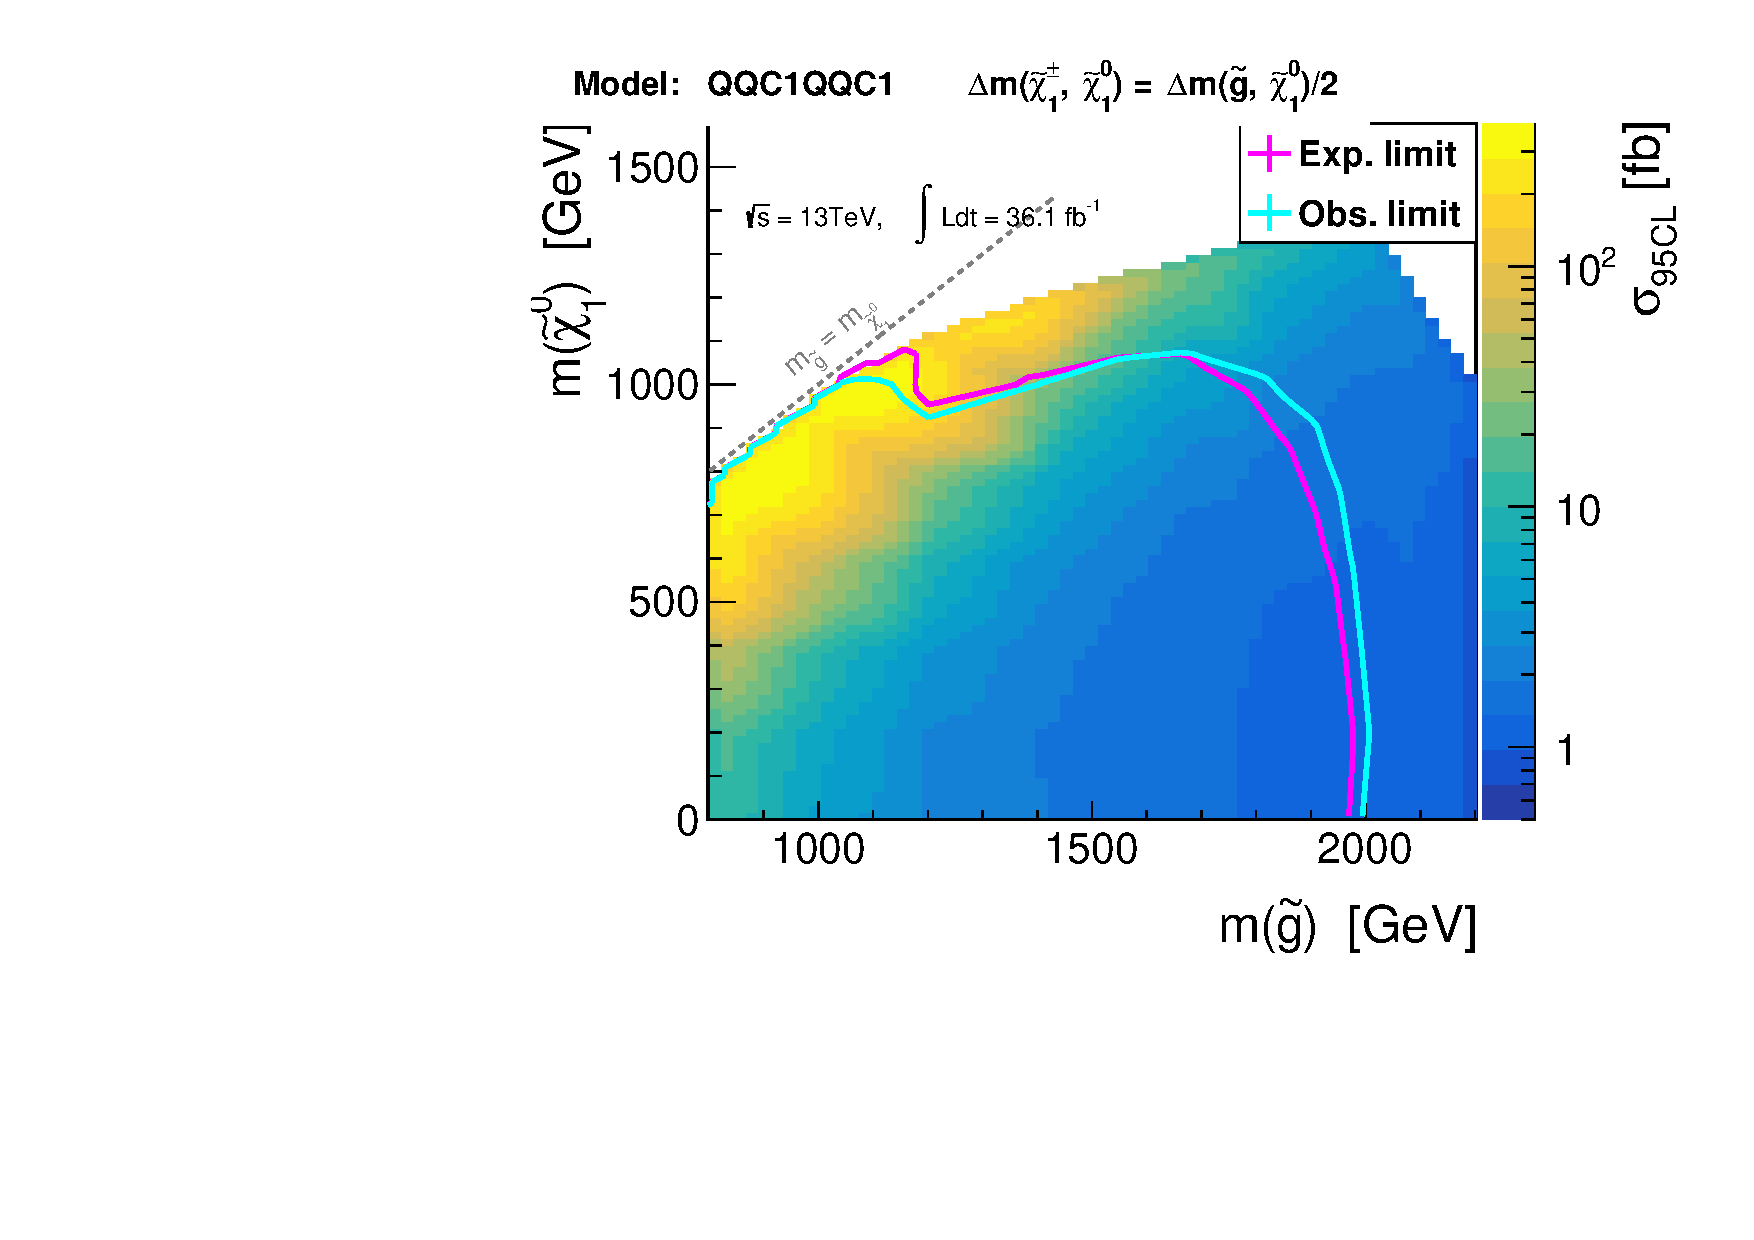
\includegraphics[width=0.48\textwidth]{figures/Result/xsecUL/symQQC1_x12.pdf}}
    \subfigure[]{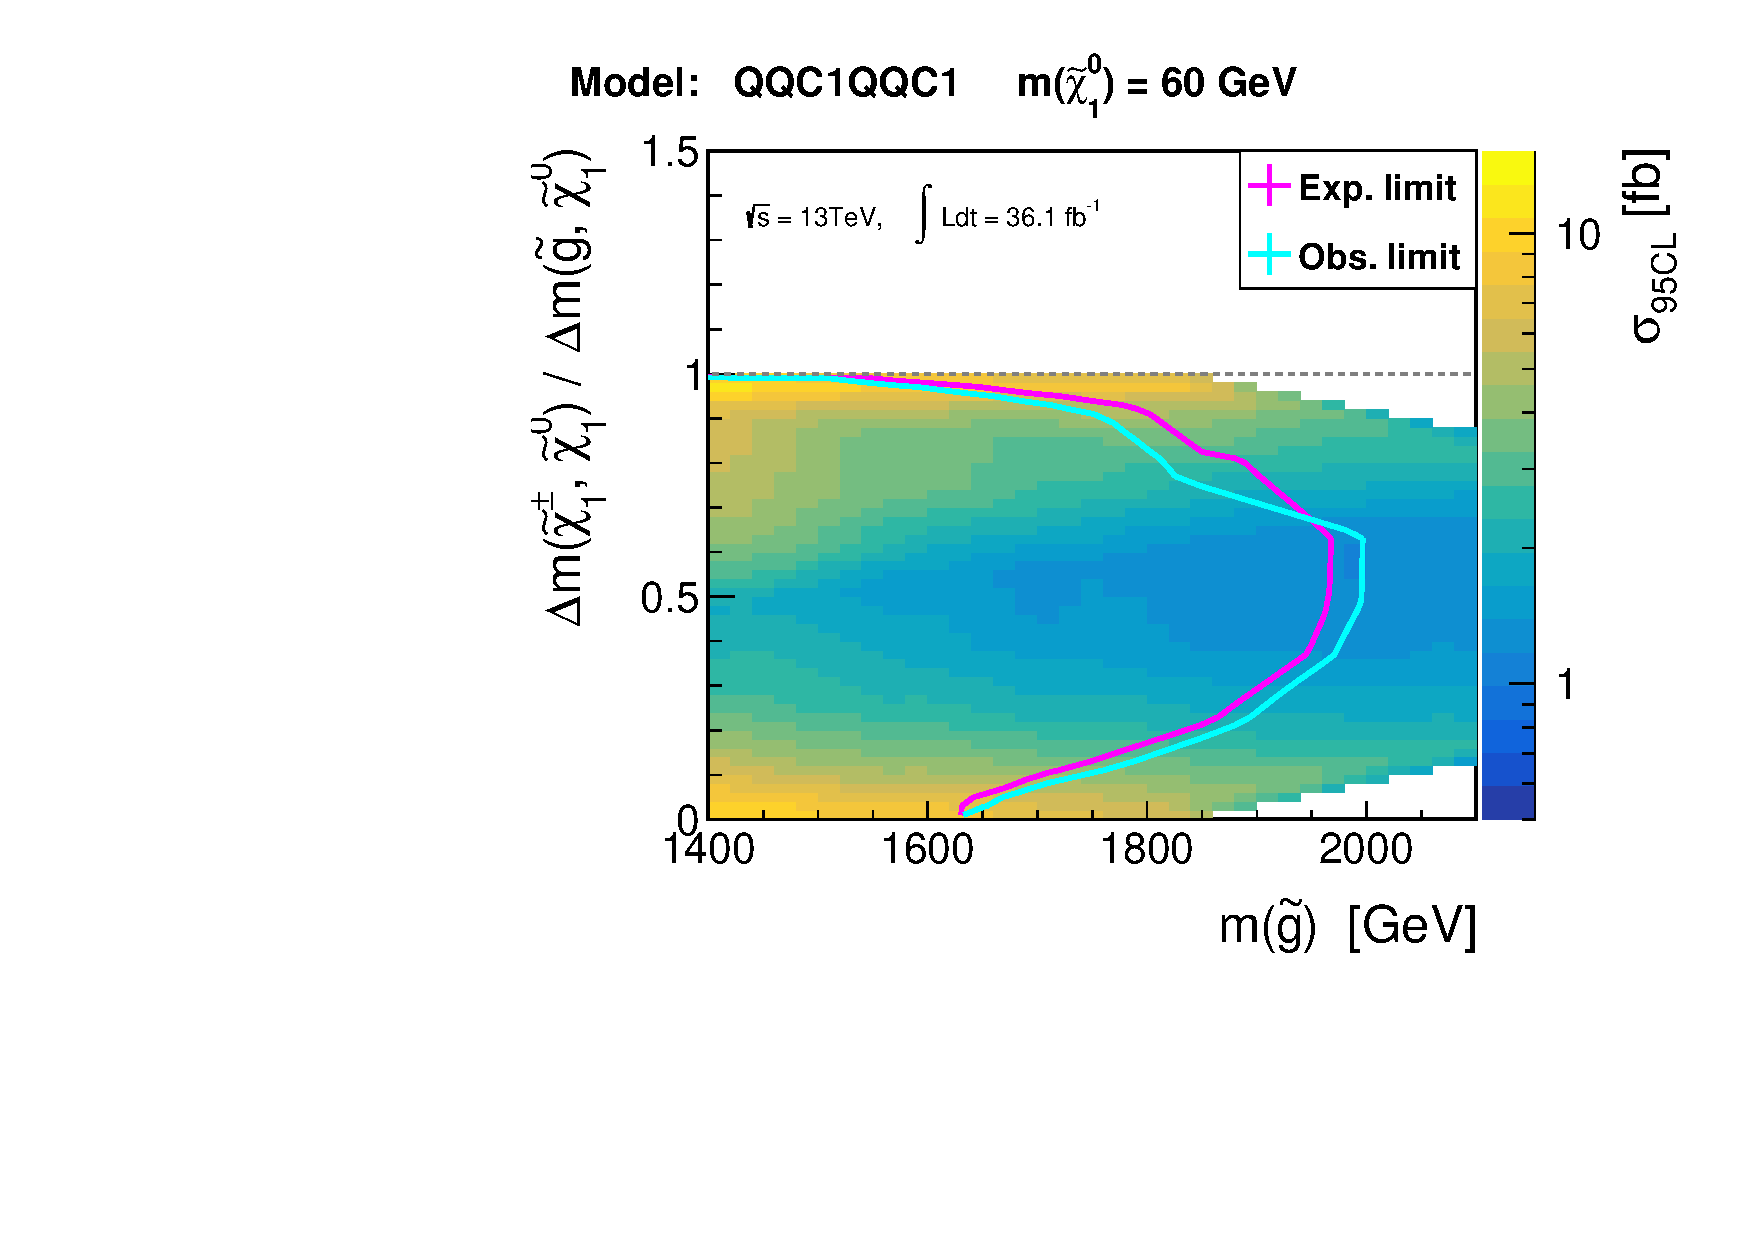
\includegraphics[width=0.48\textwidth]{figures/Result/xsecUL/symQQC1_varx.pdf}}
    \subfigure[]{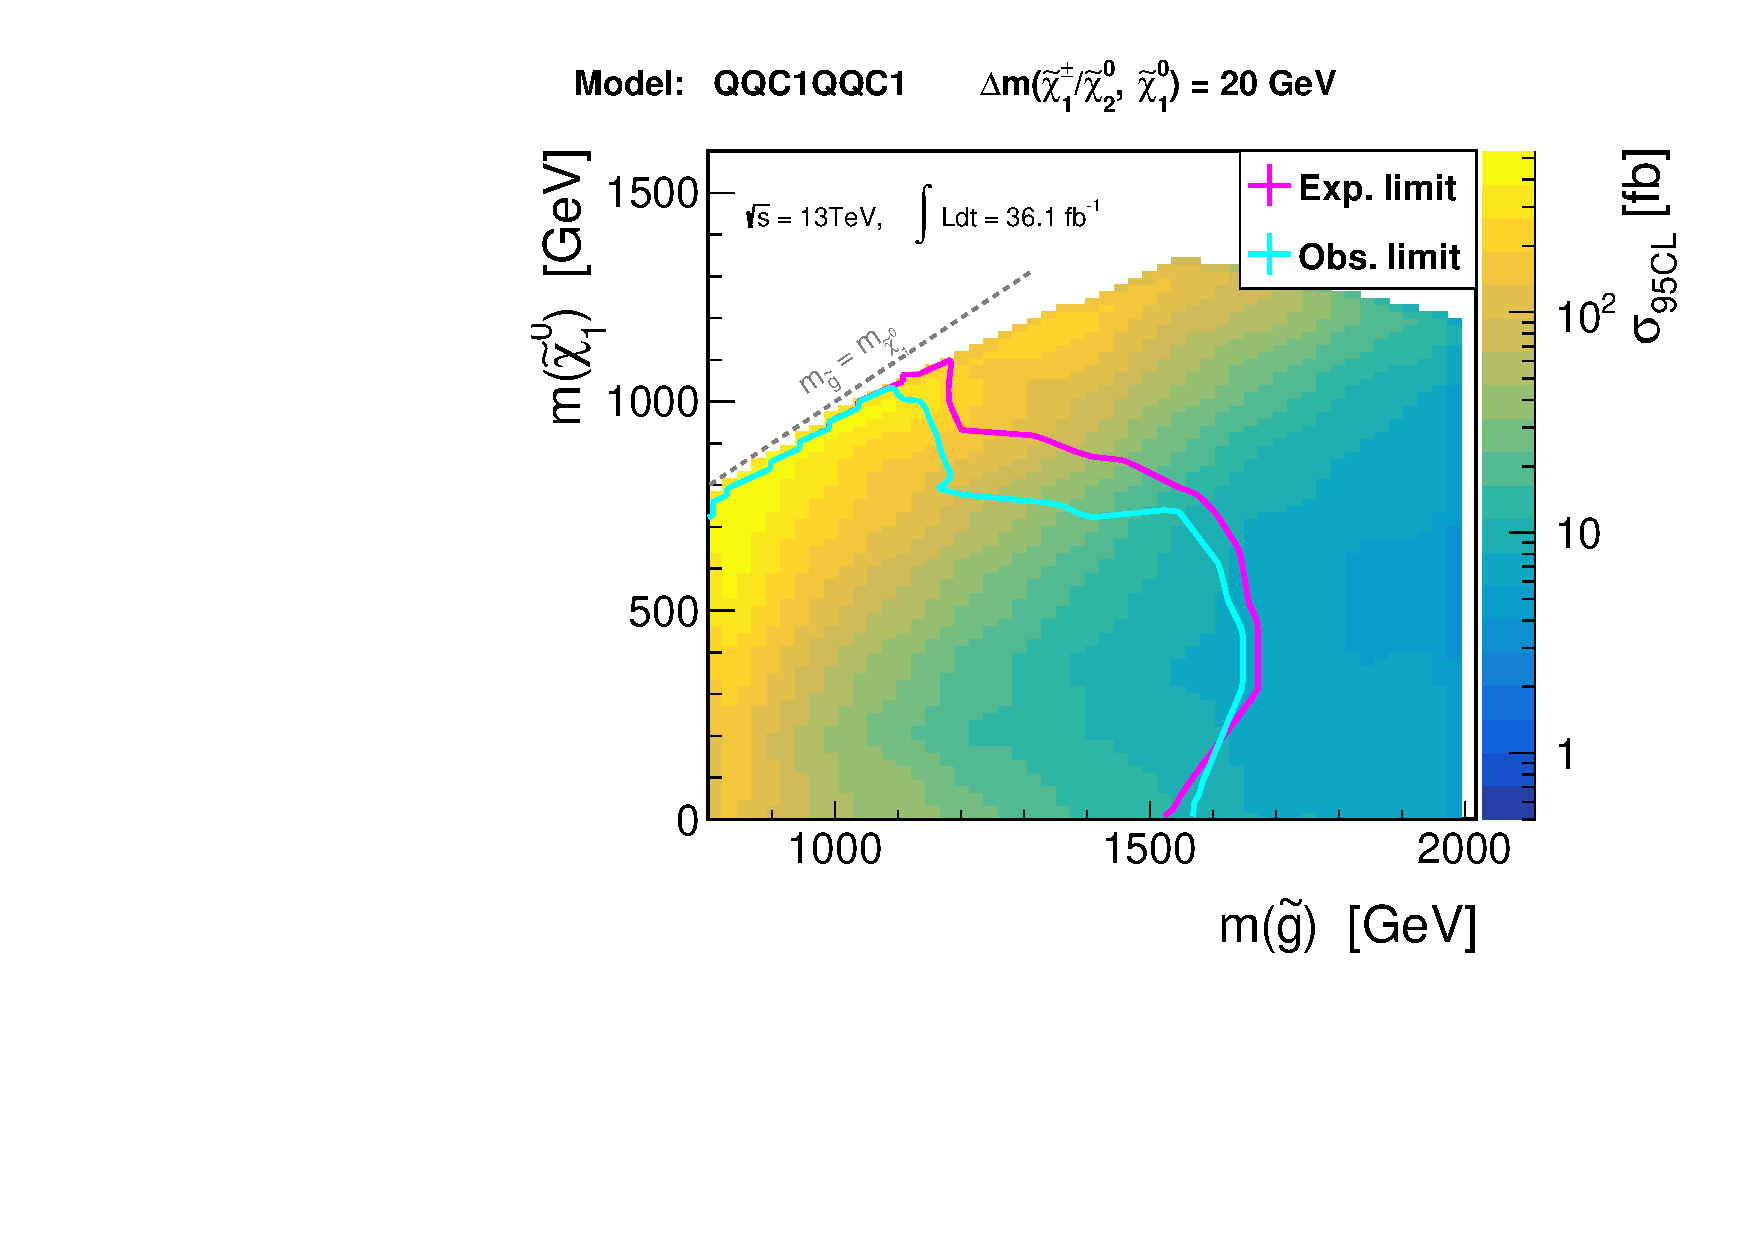
\includegraphics[width=0.48\textwidth]{figures/Result/xsecUL/symQQC1_dM20.pdf}}
    \subfigure[]{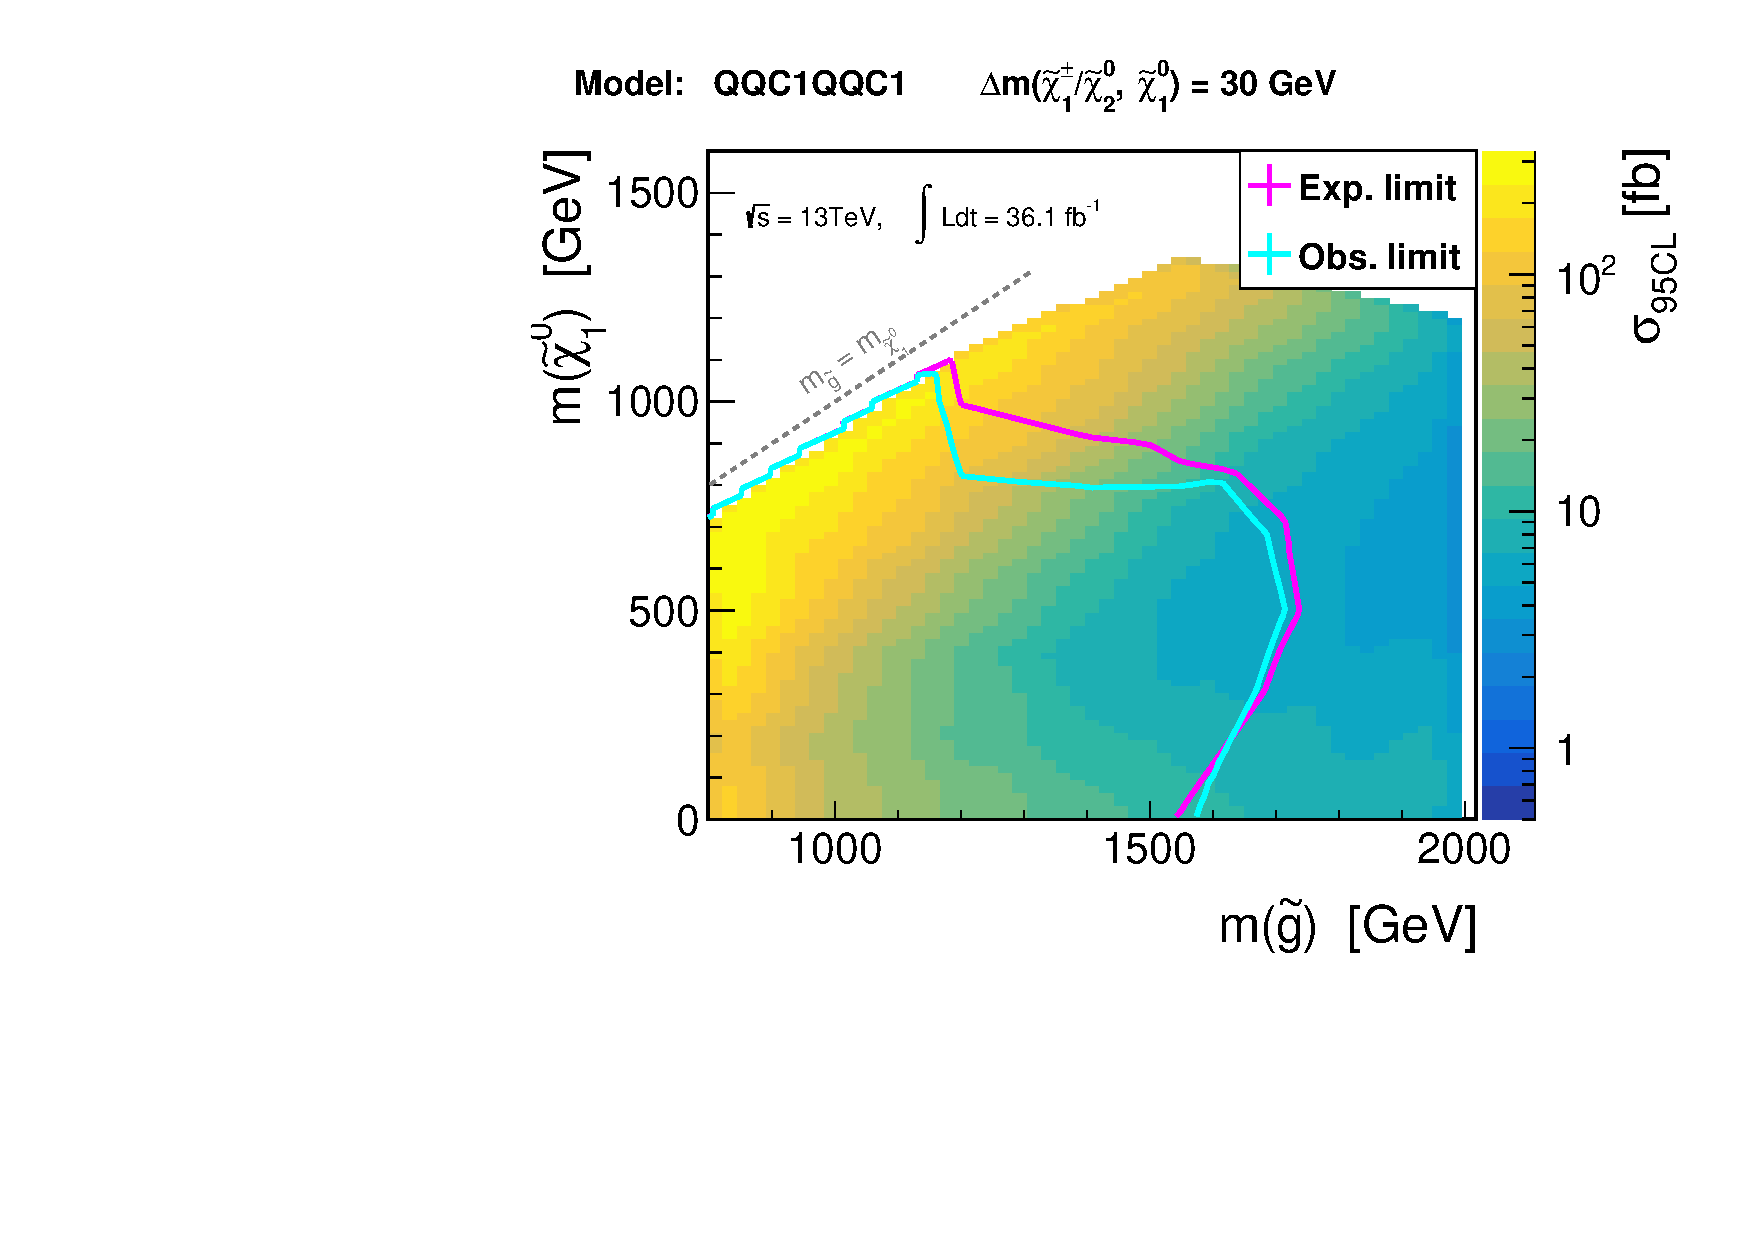
\includegraphics[width=0.48\textwidth]{figures/Result/xsecUL/symQQC1_dM30.pdf}}
    \caption{
    Upper limit of excluded cross-section (95$\%$CL) as the function of the SUSY masses, for benchmark model \textbf{QQC1QQC1}, presented in the grids (a) $x=1/2$ (b) $\mLSP=60\gev$ (c) $\dmc=20\gev$ (d) $\dmc=30\gev$.
    \label{fig::Result::xsecUL::QQC1QQC1} }
\end{figure}


%figures/Result/xsecUL/symQQC1_dM20.pdf

%% --
\begin{figure}[h]
  \centering
    \subfigure[]{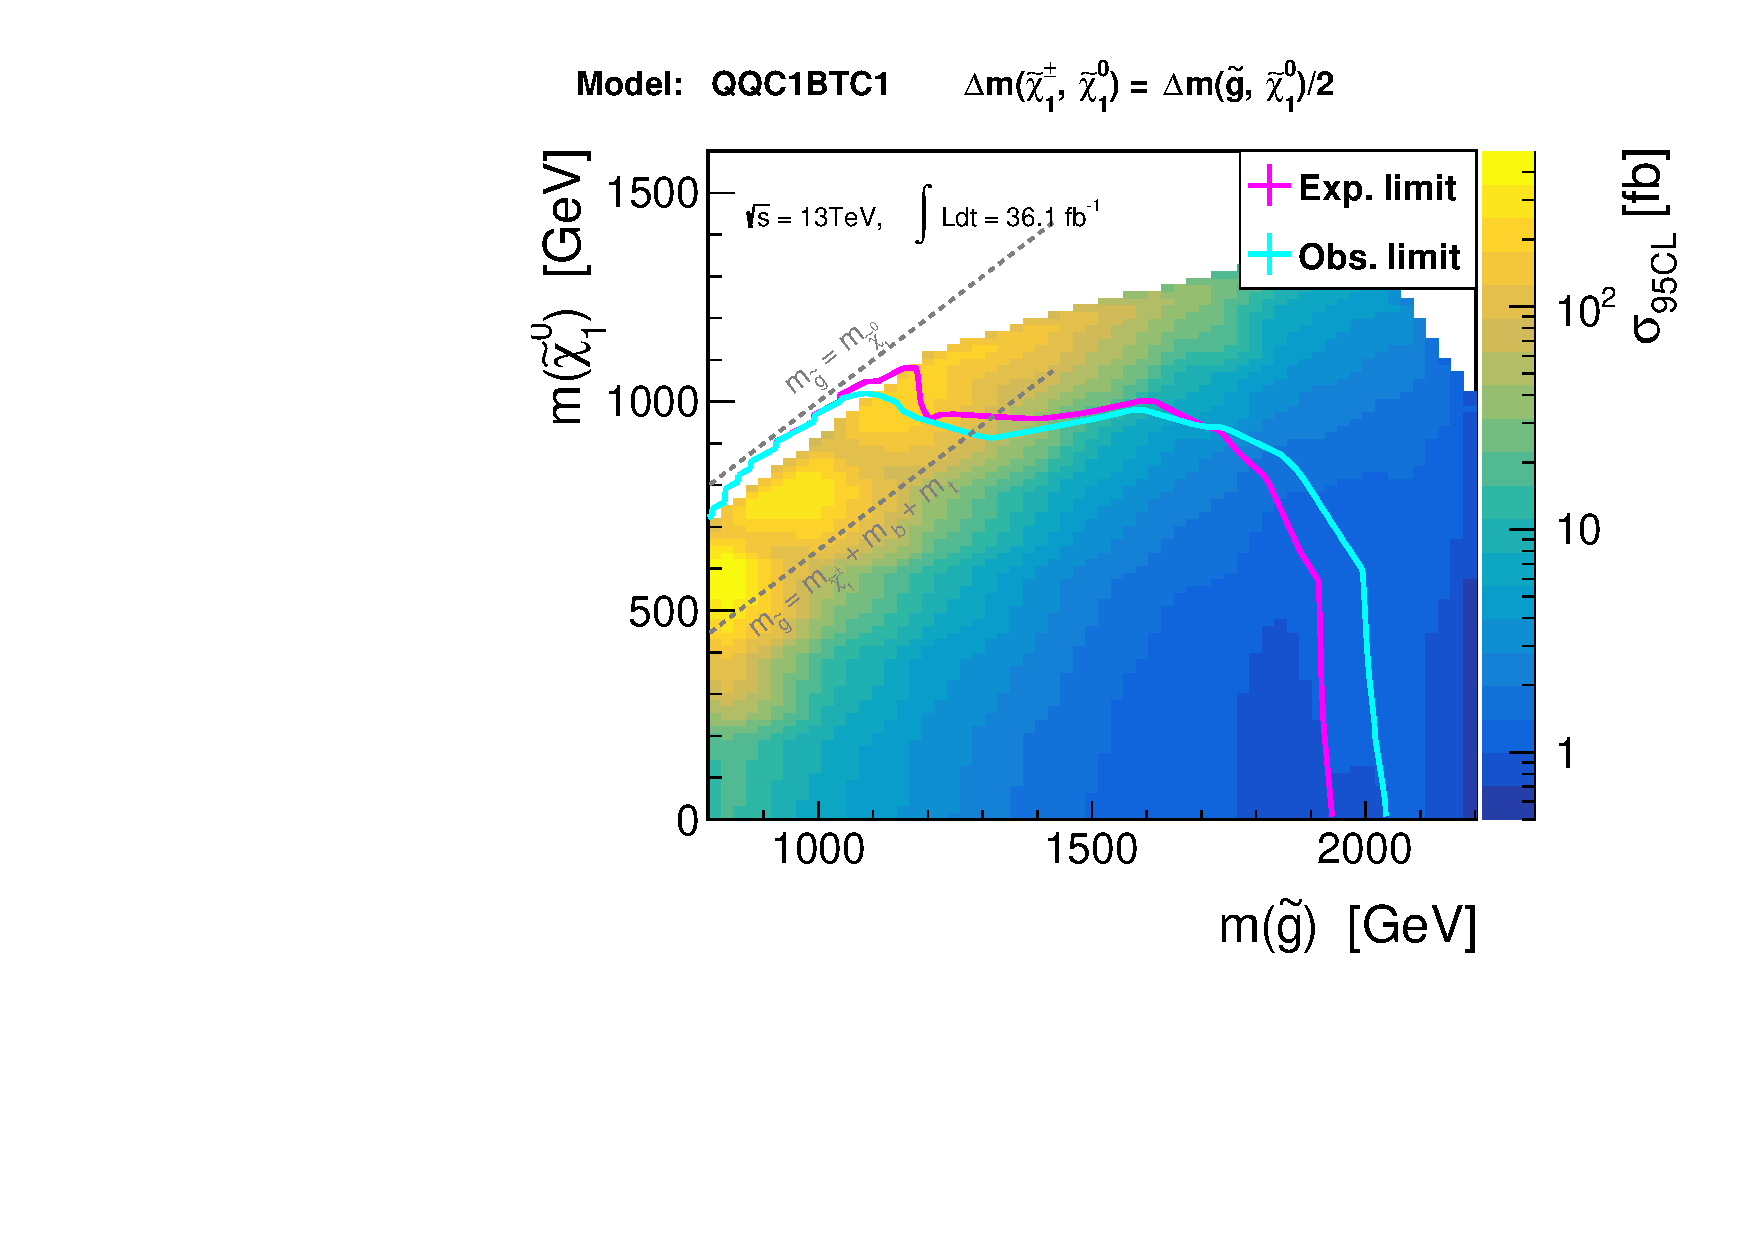
\includegraphics[width=0.48\textwidth]{figures/Result/xsecUL/QQC1BTC1_x12.pdf}}
    \subfigure[]{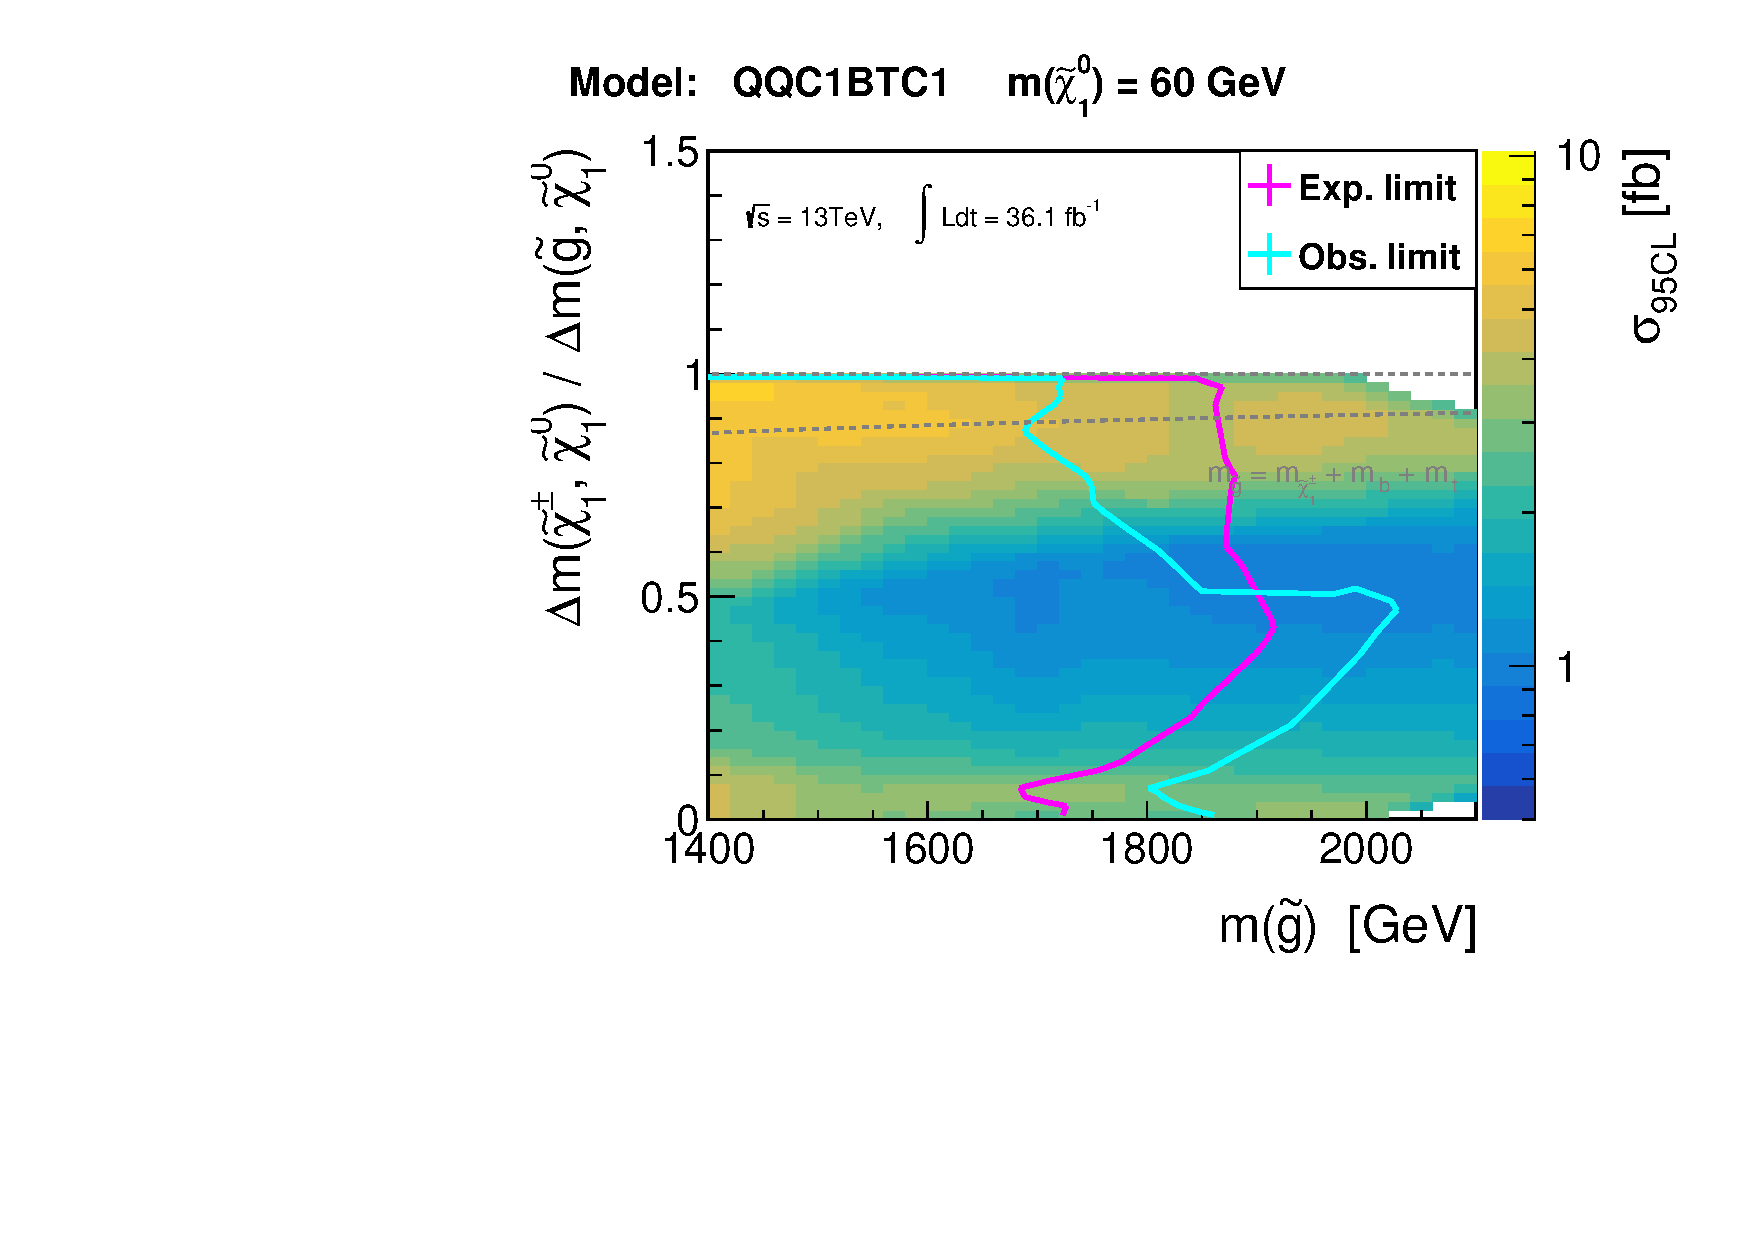
\includegraphics[width=0.48\textwidth]{figures/Result/xsecUL/QQC1BTC1_varx.pdf}}
    \subfigure[]{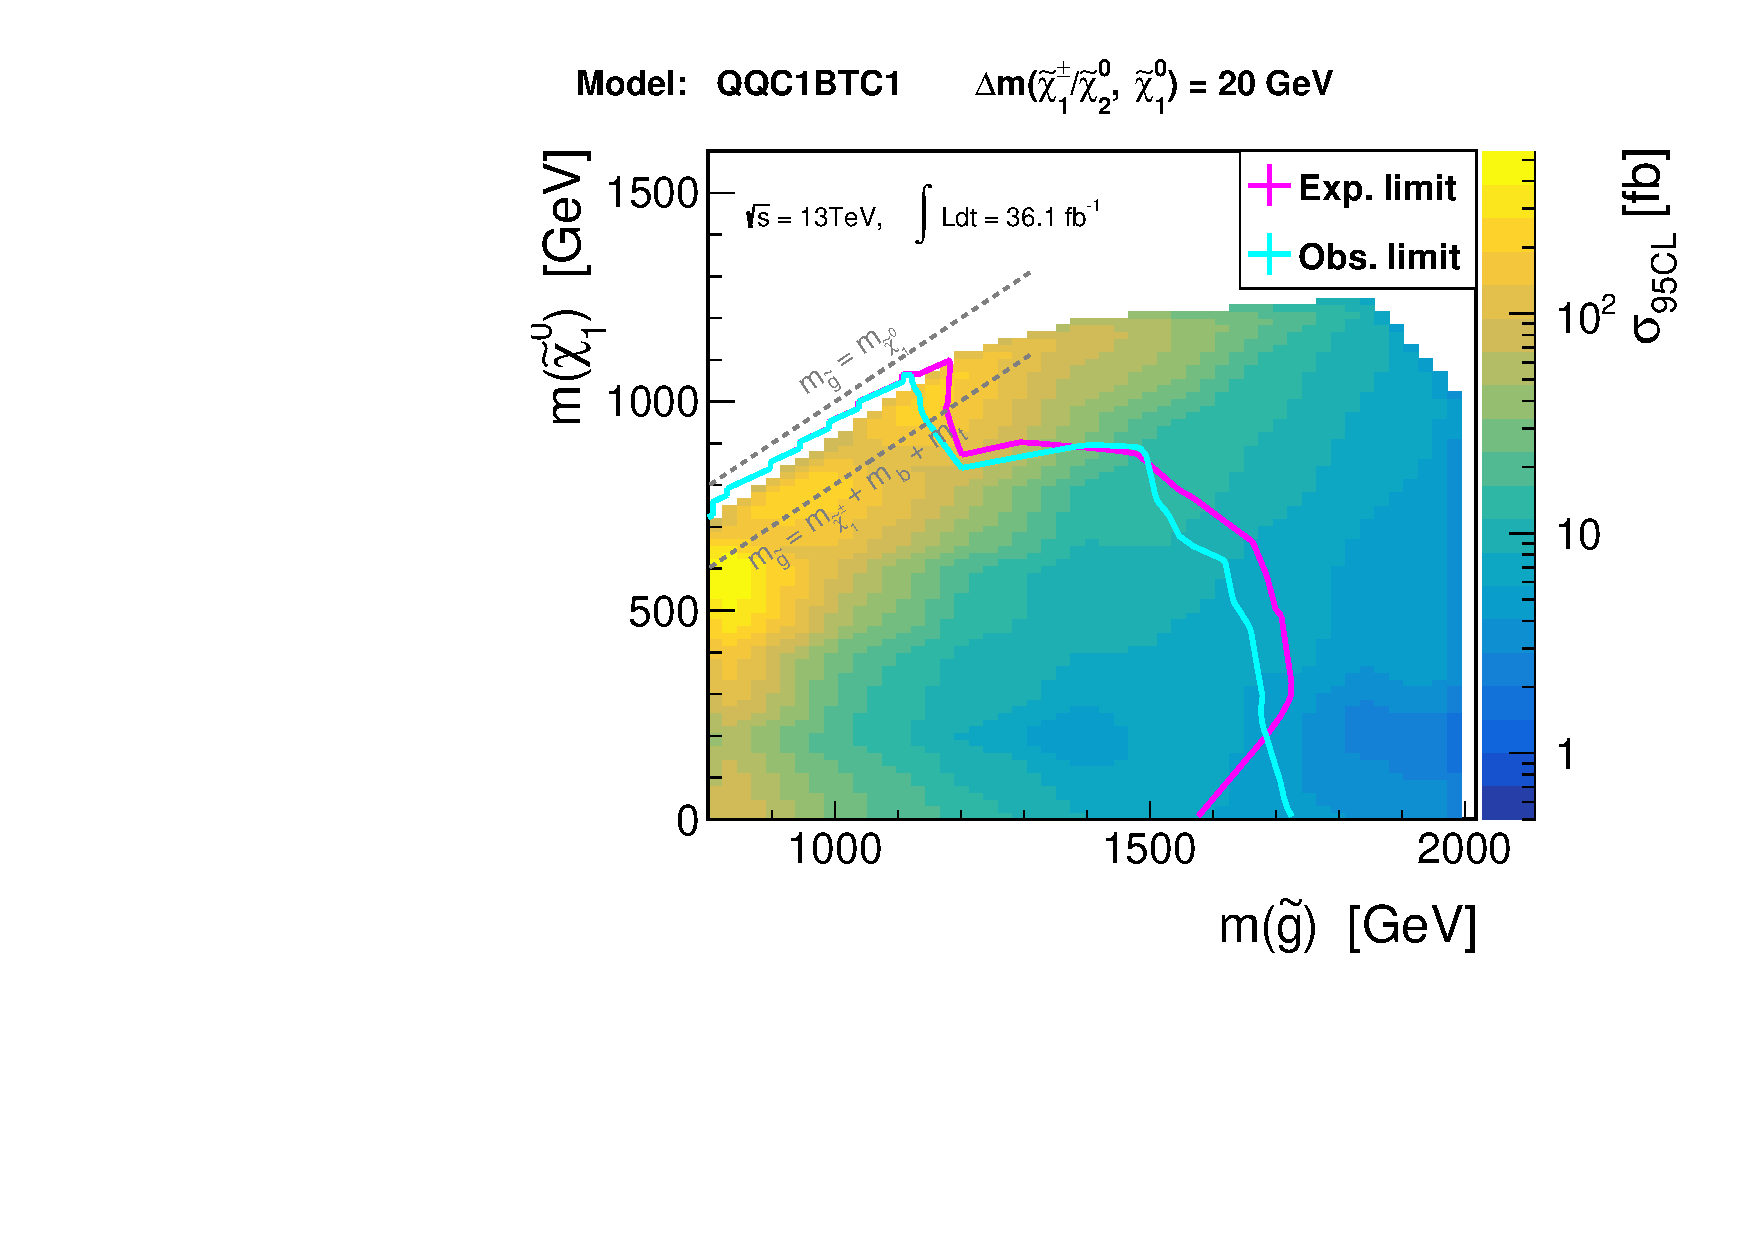
\includegraphics[width=0.48\textwidth]{figures/Result/xsecUL/QQC1BTC1_dM20.pdf}}
    \subfigure[]{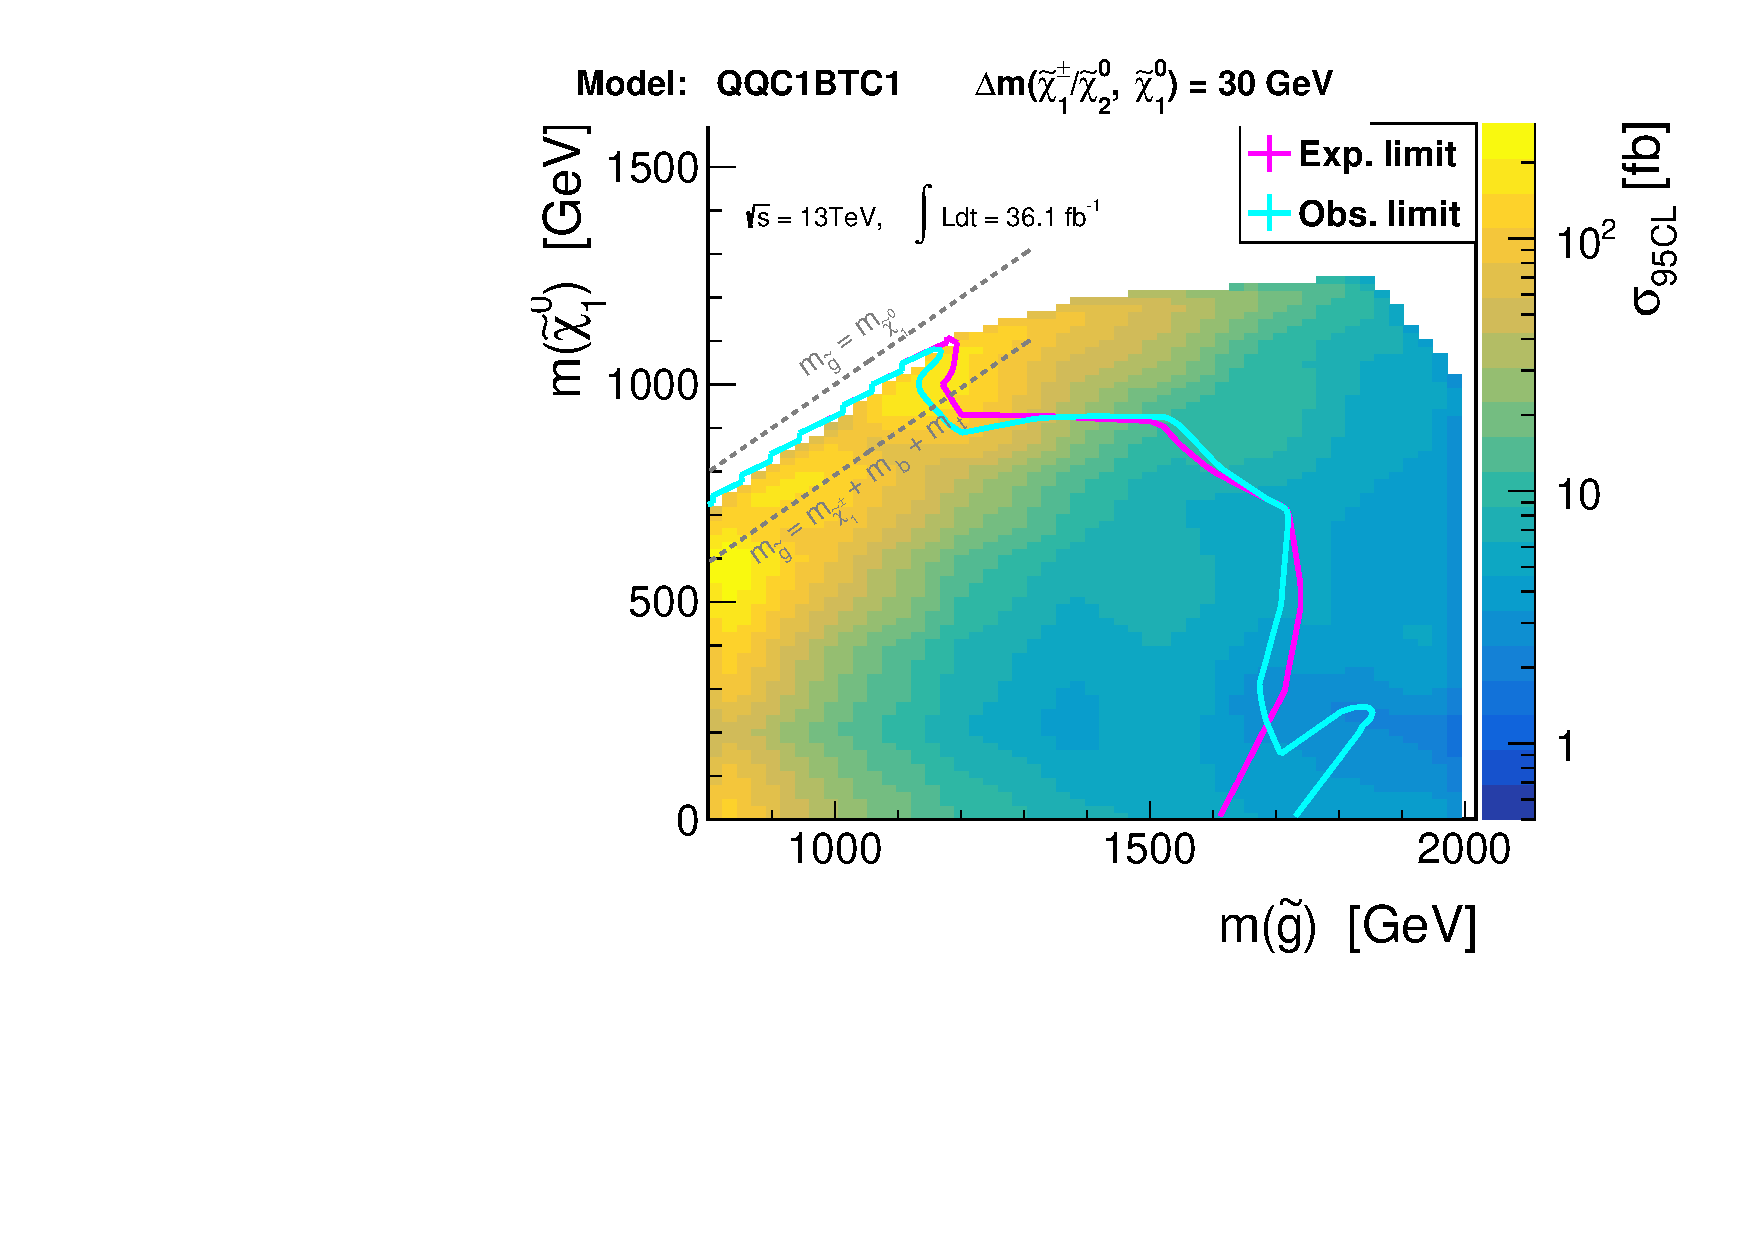
\includegraphics[width=0.48\textwidth]{figures/Result/xsecUL/QQC1BTC1_dM30.pdf}}
    \caption{
    Upper limit of excluded cross-section (95$\%$CL) as the function of the SUSY masses, for benchmark model \textbf{QQC1BTC1}, presented in the grids (a) $x=1/2$ (b) $\mLSP=60\gev$ (c) $\dmc=20\gev$ (d) $\dmc=30\gev$.
    \label{fig::Result::xsecUL::QQC1BTC1} }
\end{figure}

%% --
\begin{figure}
  \begin{center}
    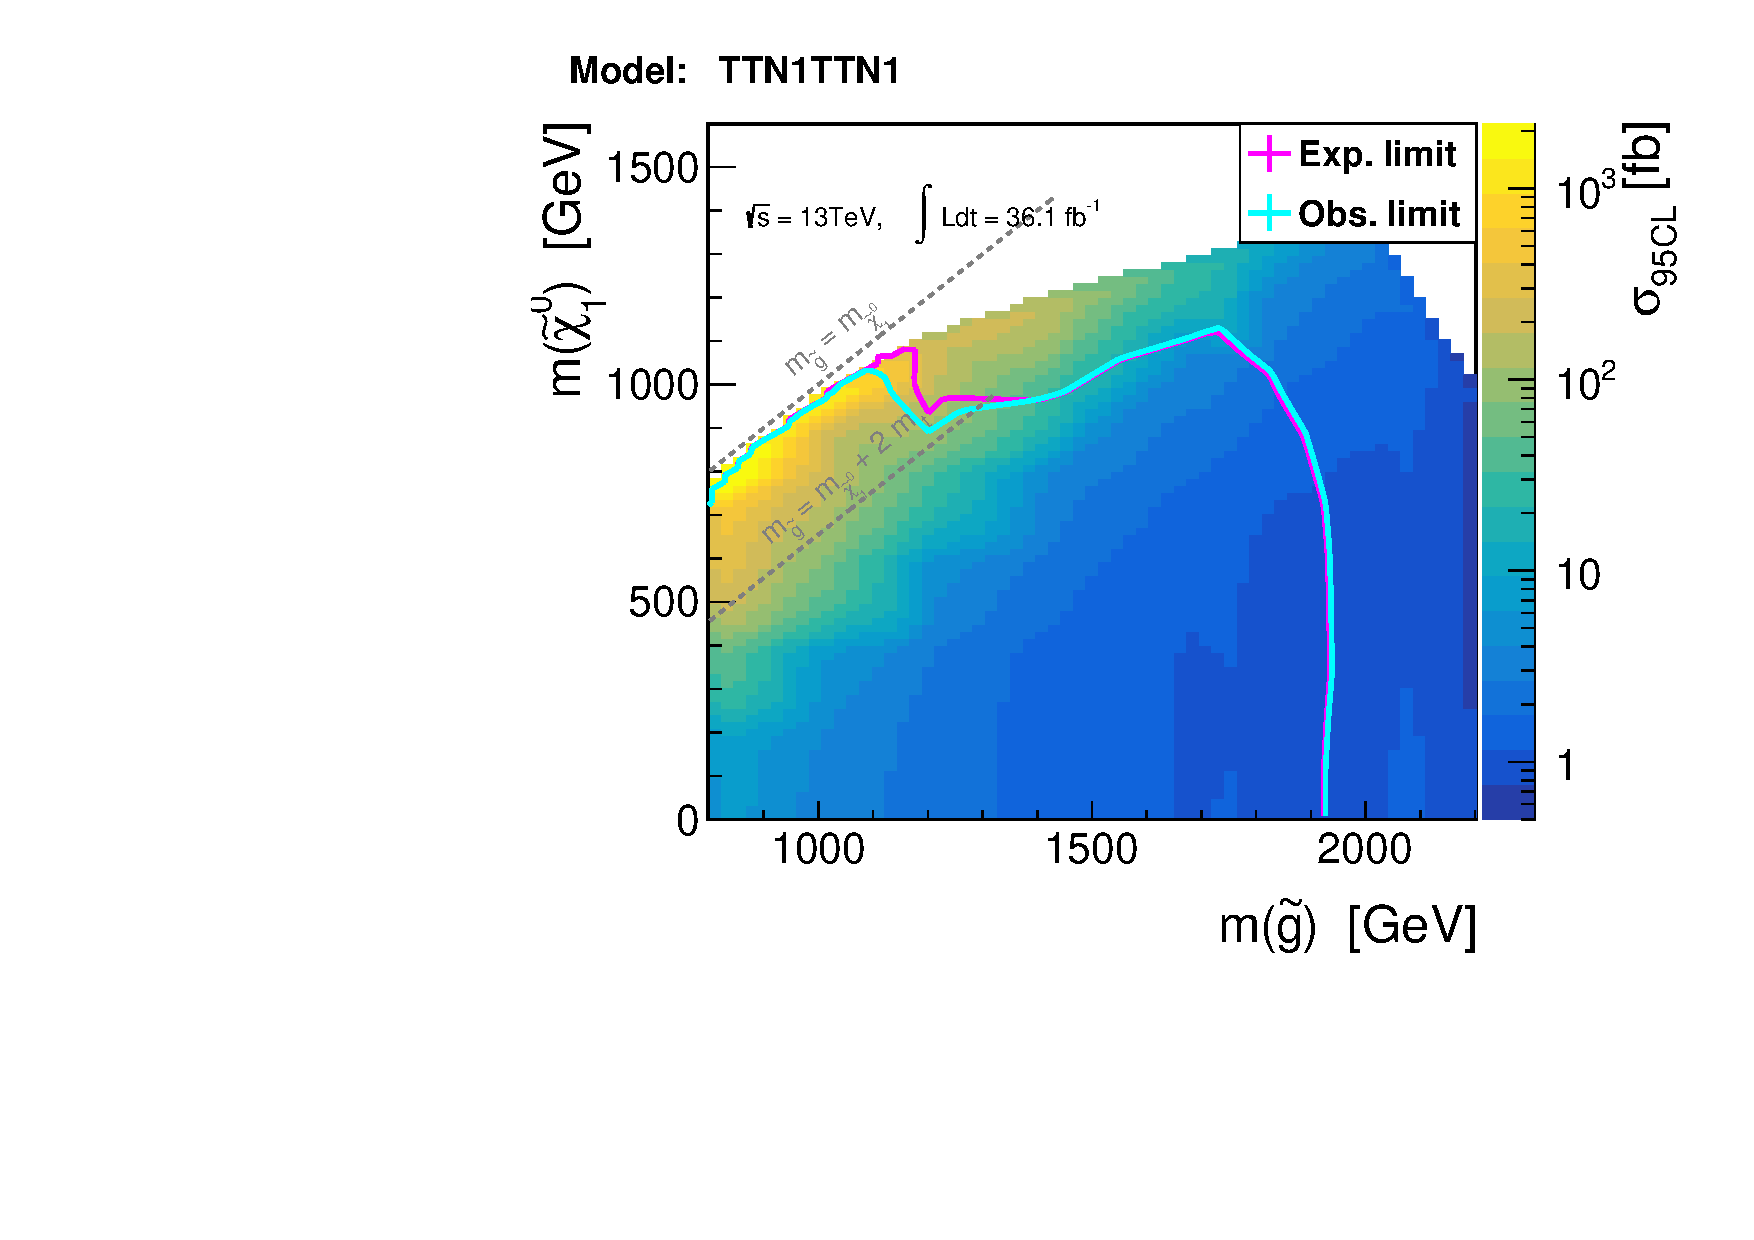
\includegraphics[width=160mm]{figures/Result/xsecUL/symTTN1_x12.pdf}
    \captionof{figure}{
    Upper limit of excluded cross-section (95$\%$CL) as the function of the SUSY masses, for benchmark model
 \textbf{TTN1TTN1}.
    \label{fig::Result::xsecUL::TTN1TTN1} }       
  \end{center}
\end{figure}
%-------------------------------                                                                                                   

